%%%%%%%%%%%%%%%%%%%%%
% 4章
%%%%%%%%%%%%%%%%%%%%%
\chapter{ヒューリスティクスを用いた手法} \label{chapter:4}

本章では,選挙区割問題を解くヒューリスティクスを作り,
その解から得られた選挙区の人口上限と下限を用いて,
ZDD構築を効率化する手法について提案する.

\section{概要}

\ref{chapter:3}章の人口制約付きZDD構築アルゴリズムでは,
パラメータとして部分グラフの重み上限$U$,下限$L$を用いた.
許容格差定数$r$では,$r$の値によって,
$U, L$の範囲が必要以上に広くなることや
$U, L$の範囲に解が一つも存在しないことがあり得る.
既存手法では,$r$の値を都道府県によって手動で調整するものがほとんどである.
そこで本研究では,選挙区割問題をヒューリスティクスで解き,
解の中で最大人口の選挙区の重みを$U$,最小人口の選挙区の重みを$L$
として定義する手法を提案する.
$U, L$が最適解に近くなればなるほど,ZDDの構築時に,
最適解でない解候補の枝刈りの回数が多くなる.
その結果,従来手法に比べて
メモリの使用量の減少及び計算時間の短縮が期待できる.

\begin{figure}[htbp]
  \centering
  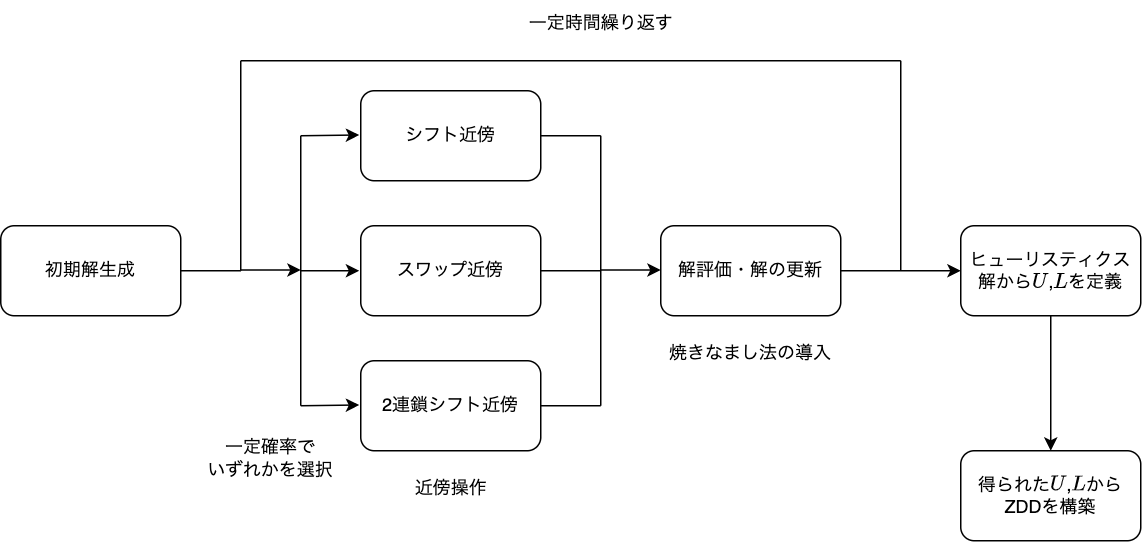
\includegraphics[scale=0.39]{img/heuristics.png}
  \caption{ヒューリスティクスを用いた提案手法}
  \label{heuristics}
\end{figure}

ヒューリスティクスでは,2.2節で定義した問題から.
評価に用いるスコアを一票の格差$\frac{\mathrm{max}(P)}{\mathrm{min}(P)}$として,
これを最小化することを目指す.

提案手法の全体像を図\ref{heuristics}に示す.
始めに選挙区割問題の初期解を生成し,次に一定の確率で
シフト近傍,スワップ近傍,2連鎖シフト近傍のいずれかを選択する.
選択した近傍操作を行って近傍解を生成し,
近傍解が選挙区割の制約(選挙区が連結であるか)を満たすか判定をする.
制約を満たしている場合には,スコアを計算し,
焼きなまし法により解の遷移を行う.
これを一定時間繰り返すことで,解を得ることができる.
その解から,$U = \mathrm{max}(P), L = \mathrm{min}(P)$
を定義し,それらを用いてZDDを構築する.
次節から,初期解生成や近傍探索のアルゴリズムについて詳細に説明する.

\section{初期解生成} \label{section:4.2}

初期解は,市区町村を表現したグラフから
選挙区を構成する部分グラフの$d$個の根を定め,
それぞれの根から幅優先探索(BFS)を行い,探索した頂点を
部分グラフに含めることで構築する.
初期解生成の擬似コードを\textbf{Algorithm 4}で示す.

\begin{breakablealgorithm}
  \caption{MakeInitialSolution}
  \label{make_initial_solution}
  \begin{algorithmic}[1]
    \Require $n, d, ave, adj\_list, w$
    \Ensure $group$
    \State $group \gets [-1] * n$
    \State $P \gets [0] * d$
    \State 頂点重みが最も大きいものから順に$d$個の頂点番号を配列$root$に保存する.
    \State $root$.reverse()
    \For {$i = 1,\ldots,d$}
      \State $queue \gets \phi $
      \State $group[root[i]] \gets i$
      \State $P[i] \gets P[i] + w[nv]$
      \State $queue$.enqueue$(root[i])$
      \While{$queue$.size() $\neq 0$ and $P[i] < ave$}
        \State $v \gets queue$.dequeue()
        \ForAll {$nv \in adj\_list[v]$}
          \If {$P[i] \geq ave$}
            \State break
          \ElsIf {$group[nv] = -1$}
            \State $group[nv] \gets i$
            \State $P[i] \gets P[i] + w[nv]$
            \State $queue$.enqueue($nv$)
          \EndIf
        \EndFor
      \EndWhile
    \EndFor
    \While{$group$の要素に$-1$が含まれる}
      \For {$vi = 1,\ldots,n$}
        \If{$group[vi]=-1$}
          \ForAll {$nv \in adj\_list[v]$}
            \If{$group[nv] \neq -1$}
              \State $group[vi] \gets group[nv]$
              \State break
            \EndIf
          \EndFor
        \EndIf
      \EndFor
    \EndWhile
    \State \textbf{return }$group$
  \end{algorithmic}
\end{breakablealgorithm}

\textbf{Algorithm 4} MakeInitialSolution の入力と出力については以下の通りである.\\
\textbf{入力}
\begin{itemize}
  \item $n$:グラフの頂点$v$の個数
  \item $d$:区割(グラフ分割)数
  \item $ave$:一選挙区の平均人口
  \item $adj\_list$:グラフの隣接リスト
  \item $w$:グラフの頂点重み
\end{itemize}
\textbf{出力}
\begin{itemize}
  \item $group$:頂点番号を添字とした配列で,
    選挙区(部分グラフ)のラベル(値は$1,\ldots,d$)が保存されている.初期値は$-1$.
\end{itemize}

2行目の$P$は部分グラフごとの重み和を保存する変数である.
配列$root$は,BFSの始点となる$d$個の頂点を含める.
3行目にもある通り,$root$は頂点重みが最も大きいものから順に指定する.
4行目で$root$を逆順にするが,これは$root$の頂点重みが小さいものから
探索を行うためである.
BFSでは,キューを用いて探索を行い,
探索した頂点を属する部分グラフに加えていく(5-22行目).
ラベル$i$の探索では,頂点$nv$を追加する際に
$group[nv]$に$i$を代入し,部分グラフの重み和$P[i]$に
$w[nv]$を加算する.
そして,重み和$P[i]$が平均重み$ave$以上になると,
その部分グラフでの探索を中断する(10,13行目).
これを全ての根$root[1],\ldots,root[d]$に対して行う.
全てのBFSを終えた後,ラベルが付かなかった($group$の値が$-1$の)
頂点に対して隣接頂点を参照し,そこからラベルを割り振る
処理を行なっている(23-34行目).
最後に$group$を出力し,これを初期解とする.

\section{近傍操作}

近傍操作とは,現在の解から少し形を変えた近傍解を生成する操作のことである.
選挙区割問題における近傍操作では,次の3つを定義する.
\begin{itemize}
  \item シフト近傍
  \item スワップ近傍
  \item 2連鎖シフト近傍
\end{itemize}

\subsection{シフト近傍}

\begin{figure}[htbp]
  \centering
  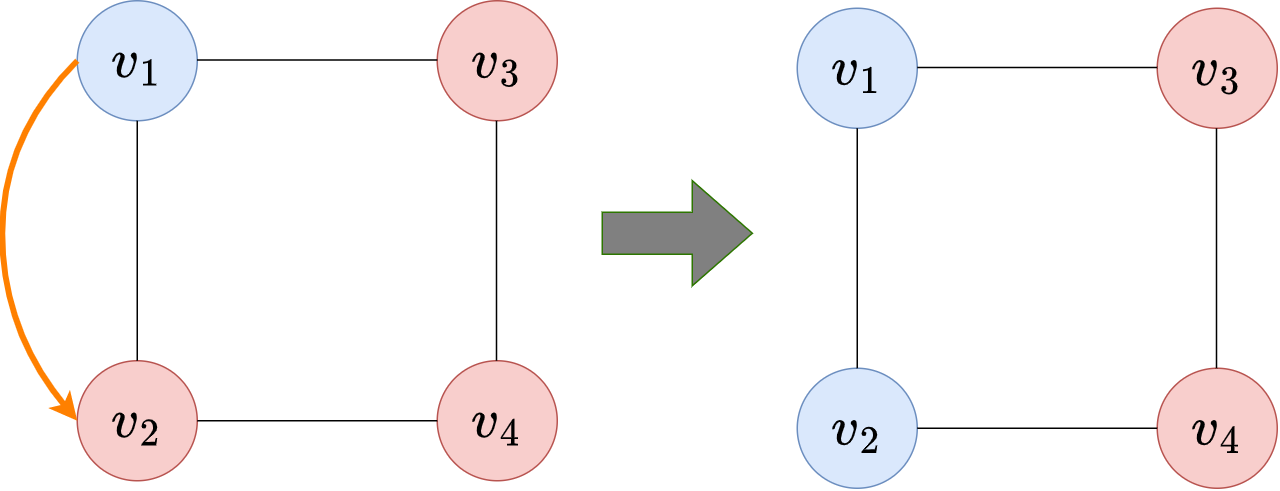
\includegraphics[scale=0.2]{img/shift-neighbor.png}
  \caption{シフト近傍}
  \label{shift-neighbor}
\end{figure}

\subsection{スワップ近傍}

\begin{figure}[htbp]
  \centering
  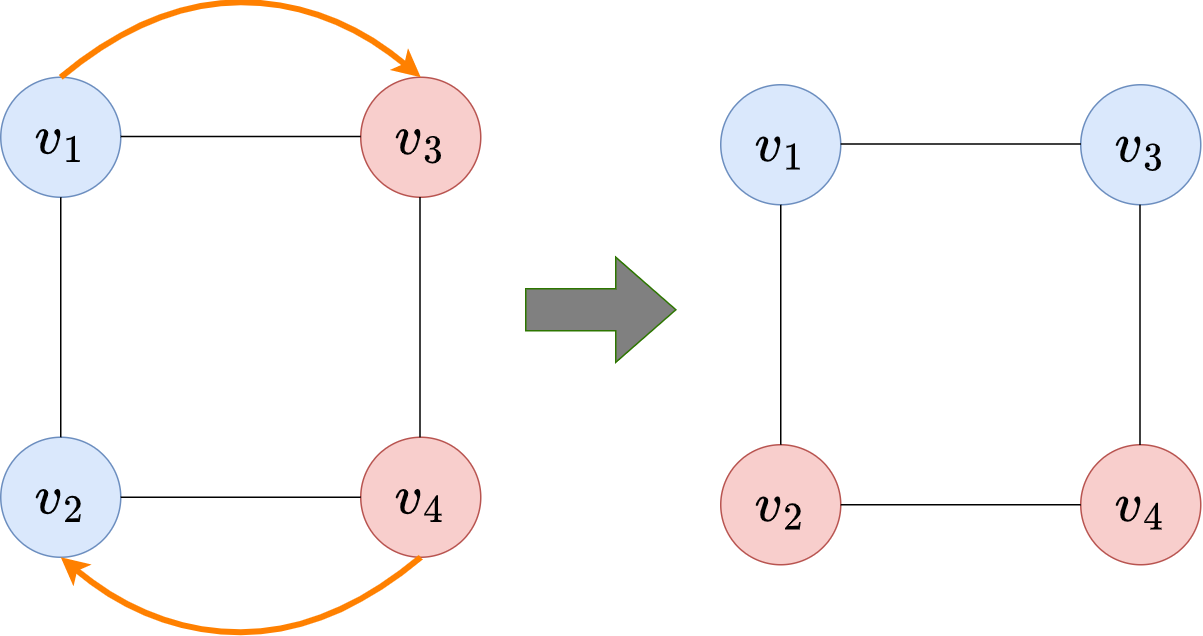
\includegraphics[scale=0.2]{img/swap-neighbor.png}
  \caption{スワップ近傍}
  \label{swap-neighbor}
\end{figure}

\subsection{2連鎖シフト近傍}

\begin{figure}[htbp]
  \centering
  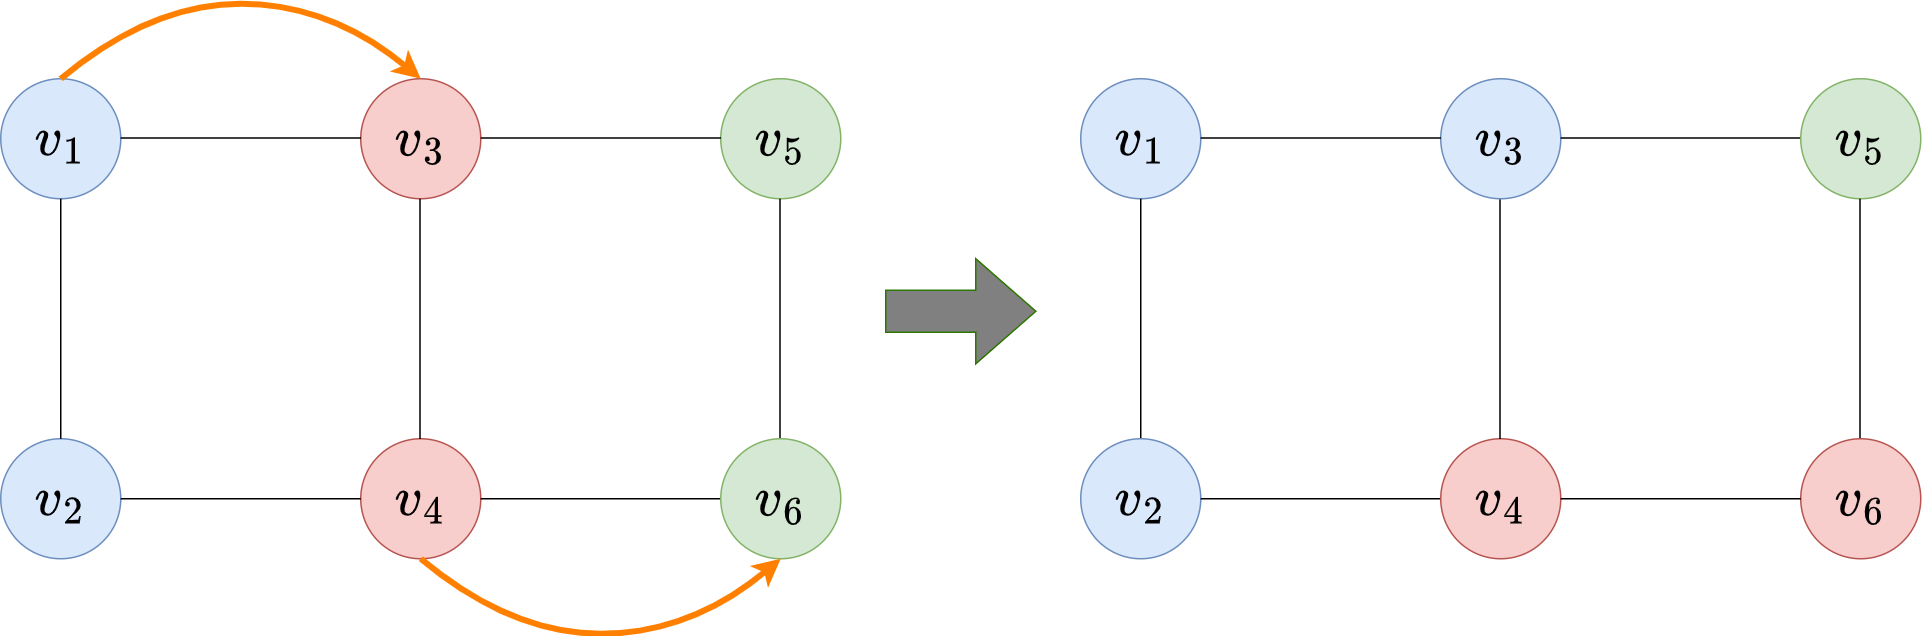
\includegraphics[scale=0.2]{img/chain-neighbor.png}
  \caption{2連鎖シフト近傍}
  \label{chain-neighbor}
\end{figure}

\section{焼きなまし法}

